\documentclass{article}
\usepackage[backend=biber,natbib=true,style=alphabetic,maxbibnames=50]{biblatex}
\addbibresource{/home/nqbh/reference/bib.bib}
\usepackage[utf8]{vietnam}
\usepackage{tocloft}
\renewcommand{\cftsecleader}{\cftdotfill{\cftdotsep}}
\usepackage[colorlinks=true,linkcolor=blue,urlcolor=red,citecolor=magenta]{hyperref}
\usepackage{amsmath,amssymb,amsthm,float,graphicx,mathtools,diagbox,tikz,tipa}
\usepackage[version=4]{mhchem}
\usepackage{enumitem}
\setlist{leftmargin=4mm}
\allowdisplaybreaks
\newtheorem{assumption}{Assumption}
\newtheorem{baitoan}{Bài toán}
\newtheorem{cauhoi}{Câu hỏi}
\newtheorem{conjecture}{Conjecture}
\newtheorem{corollary}{Corollary}
\newtheorem{dangtoan}{Dạng toán}
\newtheorem{definition}{Definition}
\newtheorem{dinhly}{Định lý}
\newtheorem{dinhnghia}{Định nghĩa}
\newtheorem{example}{Example}
\newtheorem{ghichu}{Ghi chú}
\newtheorem{hequa}{Hệ quả}
\newtheorem{hypothesis}{Hypothesis}
\newtheorem{lemma}{Lemma}
\newtheorem{luuy}{Lưu ý}
\newtheorem{nhanxet}{Nhận xét}
\newtheorem{notation}{Notation}
\newtheorem{note}{Note}
\newtheorem{principle}{Principle}
\newtheorem{problem}{Problem}
\newtheorem{proposition}{Proposition}
\newtheorem{question}{Question}
\newtheorem{remark}{Remark}
\newtheorem{theorem}{Theorem}
\newtheorem{thinghiem}{Thí nghiệm}
\newtheorem{vidu}{Ví dụ}
\usepackage[left=1cm,right=1cm,top=5mm,bottom=5mm,footskip=4mm]{geometry}

\title{Problem {\it\&} Solution Chemistry 9 Chap. 1: Inorganic Compound\\Bài Tập SGK Hóa Học 9 Chương 1: Hợp Chất Vô Cơ {\it\&} Lời Giải}
\author{Nguyễn Quản Bá Hồng\footnote{Independent Researcher, Ben Tre City, Vietnam\\e-mail: \texttt{nguyenquanbahong@gmail.com}; website: \url{https://nqbh.github.io}.}}
\date{\today}

\begin{document}
\maketitle
\tableofcontents

%------------------------------------------------------------------------------%

\section*{Lý Thuyết}
\textbf{\textsf{Phân loại các hợp chất vô cơ.}} Oxide: oxide base, e.g., CaO, \ce{Fe2O3}, oxide acid, e.g., \ce{CO2,SO2}. Acid: acid có oxygen, e.g., \ce{HNO3,H2SO4}, acid không có oxygen, e.g., HCl, HBr. Base: base tan, e.g., NaOH, KOH, base không tan \ce{Cu(OH)2,Fe(OH)3}. Muối: muối acid, e.g., \ce{KHSO4,NaHCO3}, muối trung hòa, e.g., NaCl, \ce{K2SO4}.

%------------------------------------------------------------------------------%

\section{Tính Chất Hóa Học của Oxide}

\begin{baitoan}[\cite{SGK_Hoa_Hoc_9}, 1., p. 6]
	Có 3 oxide: {\rm CaO, \ce{Fe2O3,SO3}}. Oxide nào có thể tác dụng được với: (a) nước? (b) hydrochloric acid? (c) sodium hydroxide? Viết {\rm PTHH}.
\end{baitoan}

\begin{proof}[Giải]
	(a) Các oxide tác dụng với nước: CaO, \ce{SO3}, \ce{CaO + H2O -> Ca(OH)2, SO3 + H2O -> H2SO4}. (b) Các oxide tác dụng với hydrochloric acid: CaO, \ce{Fe2O3}, \ce{CaO + $2$HCl -> CaCl2 + H2O, Fe2O3 + $6$HCl -> $2$FeCl3 + $3$H2O}. (c) Các oxide tác dụng với sodium hydroxide: \ce{SO3}, \ce{SO3 + NaOH -> NaHSO4, SO3 + $2$NaOH -> Na2SO4 + H2O}.
\end{proof}

\begin{baitoan}[\cite{SGK_Hoa_Hoc_9}, 2., p. 6]
	Có 4 chất: {\rm\ce{H2O,KOH,K2O,CO2}}. Cho biết các cặp chất có thể tác dụng với nhau.
\end{baitoan}

\begin{proof}[Giải]
	4 cặp chất có thể tác dụng với nhau: \ce{H2O} \& \ce{CO2}, \ce{H2O} \& \ce{K2O}, \ce{CO2} \& \ce{K2O}, \ce{CO2} \& KOH. PTHH: \ce{CO2 + H2O <=> H2CO3, K2O + H2O -> $2$KOH, K2O + CO2 -> K2CO3, CO2 + KOH -> KHCO3, CO2 + $2$KOH -> K2CO3 + H2O}.
\end{proof}

\begin{baitoan}[\cite{SGK_Hoa_Hoc_9}, 3., p. 6]
	Từ 5 chất: calcium oxide, sulfur (lưu huỳnh) dioxide, carbon dioxide, sulfur (lưu huỳnh) trioxide, zinc oxide, chọn chất thích hợp điền vào các sơ đồ phản ứng: (a) sulfuric acid $+$ $\ldots\to$ zinc sulfate $+$ nước. (b) sodium hydroxide $+$ $\ldots\to$ sodium sulfate $+$ nước. (c) nước $+$ $\ldots\to$ acid sulfurous. (d) nước $+$ $\ldots\to$ calcium hydroxide. (e) calcium oxide $+$ $\ldots\to$ calcium carbonate. Dùng các {\rm CTHH} để viết tất cả các {\rm PTHH} của các sơ đồ phản ứng trên.
\end{baitoan}

\begin{proof}[Giải]
	(a) sulfuric acid $+$ zinc oxide $\to$ zinc sulfate $+$ nước: \ce{H2SO4 + ZnO -> ZnSO4 + H2O}. (b) sodium hydroxide $+$ lưu huỳnh trioxide $\to$ sodium sulfate $+$ nước: \ce{$2$NaOH + SO3 -> Na2SO4 + H2O}. (c) nước $+$ lưu huỳnh dioxide $\to$ acid sulfurous: \ce{H2O + SO2 <=> H2SO3}. (d) nước $+$ calcium oxide $\to$ calcium hydroxide: \ce{H2O + CaO -> Ca(OH)2}. (e) calcium oxide $+$ carbon dioxide $\to$ calcium carbonate: \ce{CaO + CO2 -> CaCO3 v}.
\end{proof}

\begin{baitoan}[\cite{SGK_Hoa_Hoc_9}, 4., p. 6]
	Cho 5 oxide: {\rm\ce{CO2,SO2,Na2O,CaO,CuO}}. Chọn các chất tác dụng được với: (a) nước, tạo thành dung dịch acid. (b) nước, tạo thành dung dịch base. (c) dung dịch acid, tạo thành muối \& nước. (d) dung dịch base, tạo thành muối \& nước. Viết {\rm PTHH}.
\end{baitoan}

\begin{proof}[Giải]
	(a) \ce{CO2,SO2} tác dụng với nước tạo thành dung dịch acid: \ce{CO2 + H2O <=> H2CO3, SO2 + H2O <=> H2SO3}. (b) \ce{Na2O}, CaO tác dụng với nước tạo thành dung dịch base: \ce{Na2O + H2O -> $2$NaOH, CaO + H2O -> Ca(OH)2}. (c) \ce{Na2O}, CaO, CuO tác dụng với dung dịch acid tạo thành muối \& nước: \ce{Na2O + $2$HCl -> $2$HCl + H2O, CaO + $2$HNO3 -> Ca(NO3)2 + H2O, CuO + H2SO4 -> CuSO4 + H2O}. (d) \ce{CO2,SO2} tác dụng với dung dịch base tạo thành muối \& nước: \ce{CO2 + Ca(OH)2 -> CaCO3 v + H2O, SO2 + Ca(OH)2 -> CaSO3 v + H2O}.
\end{proof}

\begin{baitoan}[\cite{SGK_Hoa_Hoc_9}, 5., p. 6]
	Có hỗn hợp khí {\rm\ce{CO2,O2}}. Làm thế nào để có thể thu được khí {\rm\ce{O2}} từ hỗn hợp trên? Trình bày cách làm \& viết  {\rm PTHH}.
\end{baitoan}

\begin{proof}[1st giải]
	\cite[p. 7]{Ninh_giai_BT_Hoa_Hoc_9}: Trong số các khí \& hơi của hỗn hợp, có 1 oxide acid là \ce{CO2}. Theo tính chất hóa học của oxide acid, chất này phản ứng với kiềm tạo thành muối \& nước. Chất khí oxygen không có tính chất này. Do đó ta chọn dung dịch \ce{Ca(OH)2} để tách riêng khí oxygen ra khỏi hỗn hợp. Cách làm: \textit{Bước 1}: Cho hỗn hợp khí đi qua bình đựng dung dịch \ce{Ca(OH)2} dư, toàn bộ khí \ce{CO2} trong hỗn hợp sẽ phản ứng \& oxygen đi qua vì không phản ứng. PTHH: \ce{CO2 + Ca(OH)2 -> CaCO3 v + H2O}. \textit{Bước 2}: Khí oxygen có lẫn 1 ít hơi nước (nước vôi trong chưa hấp thụ hết) ta dẫn qua bình đựng dung dịch acid sulfuric đặc. Hơi nước bị acid giữ lại, ta được khí oxygen sạch.
\end{proof}

\begin{proof}[2nd giải]
	Dẫn hỗn hợp khí \ce{CO2,O2} đi qua bình đựng dung dịch kiềm lấy dư, e.g., \ce{Ca(OH)2}, NaOH, $\ldots$, khí \ce{CO2} bị hấp thụ hết do có phản ứng với kiềm: \ce{CO2 + Ca(OH)2 -> CaCO2 v + H2O} hoặc \ce{CO2 + $2$NaOH -> Na2CO3 + H2O}. Khí thoát ra khỏi bình chỉ có \ce{O2} nên sẽ thu được khí \ce{O2}.
\end{proof}

\begin{baitoan}[\cite{SGK_Hoa_Hoc_9}, 6., p. 6]
	Cho {\rm1.6 g} copper {\rm(II)} oxide tác dụng với {\rm100 g} dung dịch acid sulfuric có nồng độ $20\%$. (a) Viết PTHH. (b) Tính nồng độ \% của các chất có trong dung dịch sau khi phản ứng kết thúc.
\end{baitoan}

\begin{proof}[1st giải]
	(a) $n_{\rm CuO} = \dfrac{1.6}{80} = 0.02$ mol, $n_{\ce{H2SO4}} = \dfrac{100\cdot20\%}{98} = \dfrac{10}{49}\approx0.204 > 0.02\Rightarrow$ \ce{H2SO4} dư, CuO phản ứng hết. PTHH: \ce{CuO + H2SO4 -> CuSO4 + H2O} với $n_{\rm CuO} = n_{\ce{H2SO4}\footnotesize\mbox{pư}} = n_{\ce{CuSO4}} = 0.02$ mol. (b) $C\%_{\ce{CuSO4}} = \dfrac{0.02\cdot160}{1.6 + 100}\cdot100\%\approx3.15\%$, $C\%_{\ce{H2SO4}} = \dfrac{20 - 0.02\cdot98}{1.6 + 100}\cdot100\%\approx17.756\%$.
\end{proof}

\begin{proof}[2nd giải]
	$m_{\ce{H2SO4}} = m_{\rm dd\ce{H2SO4}}C\% = 100\cdot20\% = 20$ g, $n_{\rm CuO} = \dfrac{m_{\rm CuO}}{M_{\rm CuO}} = \dfrac{1.6}{80} = 0.02$ mol, $n_{\ce{H2SO4}} = \dfrac{m_{\ce{H2SO4}}}{M_{\ce{H2SO4}}} = \dfrac{20}{98} = \dfrac{10}{49}$ mol. (a) PTHH: \ce{CuO + H2SO4 -> CuSO4 + H2O}. Vì $n_{\rm CuO} < n_{\ce{H2SO4}}$ ($0.02 < \frac{10}{49}\approx0.204$) nên CuO phản ứng hết, \ce{H2SO4} dư, suy ra khối lượng \ce{CuSO4} tạo thành \& \ce{H2SO4} phản ứng tính theo số mol CuO. (b) Dung dịch sau phản ứng có 2 chất tan: \ce{CuSO4} \& \ce{H2SO4} còn dư. $C\%_{\ce{CuSO4}} = \dfrac{m_{\ce{CuSO4}}}{m_{\rm dd}}\cdot100\% = \dfrac{0.02\cdot160}{1.6 + 100}\cdot100\%\approx3.15\%$. $C\%_{\ce{H2SO4}} = \dfrac{m_{\ce{H2SO4}\footnotesize\mbox{dư}}}{m_{\rm dd}}\cdot100\% = \dfrac{20 - 0.02\cdot98}{1.6 + 100}\cdot100\%\approx17.756\%$.
\end{proof}

\begin{baitoan}[Mở rộng \cite{SGK_Hoa_Hoc_9}, 6., p. 6]
	Cho $m_1$ {\rm g} copper {\rm(II)} oxide tác dụng với $m_2$ {\rm g} dung dịch acid sulfuric có nồng độ $C\%$. Tính nồng độ \% của các chất có trong dung dịch sau khi phản ứng kết thúc theo $m_1,m_2,C\%$ biết sẽ lọc ra {\rm CuO} khỏi dung dịch nếu {\rm CuO} dư.
\end{baitoan}

\begin{proof}[Giải]
	$m_{\ce{H2SO4}} = m_{\rm dd\ce{H2SO4}}C\% = m_2C\%$ g, $n_{\rm CuO} = \dfrac{m_{\rm CuO}}{M_{\rm CuO}} = \dfrac{m_1}{80}$ mol, $n_{\ce{H2SO4}} = \dfrac{m_{\ce{H2SO4}}}{M_{\ce{H2SO4}}} = \dfrac{m_2C\%}{98}$ mol. PTHH: \ce{CuO + H2SO4 -> CuSO4 + H2O}. Vì nếu CuO dư sẽ bị lọc ra, nên theo định luật bảo toàn khối lượng, $m_{\rm dd} = m_{\rm CuO\footnotesize\mbox{pư}} + m_{\rm dd\ce{H2SO4}}$ g. Xét 2 trường hợp:
	\begin{itemize}
		\item[(a)] Nếu $n_{\rm CuO} < n_{\ce{H2SO4}}$, i.e., nếu $m_1,m_2,C\%$ thỏa $\dfrac{m_1}{80} < \dfrac{m_2C\%}{98}$ thì CuO phản ứng hết, \ce{H2SO4} dư, suy ra $n_{\rm CuO} = n_{\ce{H2SO4}\footnotesize\mbox{pư}} = n_{\ce{CuSO4}} = \dfrac{m_1}{80}$ mol, $m_{\ce{H2SO4}\footnotesize\mbox{dư}} = m_{\ce{H2SO4}} - m_{\ce{H2SO4}\footnotesize\mbox{pư}} = m_2C\% - 98\dfrac{m_1}{80}$. Dung dịch sau phản ứng có 2 chất tan: \ce{CuSO4} \& \ce{H2SO4} còn dư.
		\begin{align*}
			C\%_{\ce{CuSO4}} &= \frac{m_{\ce{CuSO4}}}{m_{\rm dd}}\cdot100\% = \frac{\frac{m_1}{80}\cdot160}{m_1 + m_2}\cdot100\% = \frac{200m_1}{m_1 + m_2}\%,\\
			C\%_{\ce{H2SO4}} &= \frac{m_{\ce{H2SO4}\footnotesize\mbox{dư}}}{m_{\rm dd}}\cdot100\% = \frac{100\left(m_2C\% - \dfrac{98m_1}{80}\right)}{m_1 + m_2}\% = \frac{100m_2C\% - 122.5m_1}{m_1 + m_2}\%.
		\end{align*}
		\item[(b)] Nếu $n_{\rm CuO} = n_{\ce{H2SO4}}$, i.e., nếu $m_1,m_2,C\%$ thỏa $\dfrac{m_1}{80} = \dfrac{m_2C\%}{98}$ thì cả CuO \& \ce{H2SO4} đều phản ứng hết. Dung dịch sau phản ứng có duy nhất 1 chất tan \ce{CuSO4} \& $n_{\ce{CuSO4}} = n_{\rm CuO} = n_{\ce{H2SO4}} = \dfrac{m_1}{80}$:
		\begin{align*}
			C\%_{\ce{CuSO4}} &= \frac{m_{\ce{CuSO4}}}{m_{\rm dd}}\cdot100\% = \frac{\frac{m_1}{80}\cdot160}{m_1 + m_2}\cdot100\% = \frac{200m_1}{m_1 + m_2}\%.
		\end{align*}
		\item[(c)] Nếu $n_{\rm CuO} > n_{\ce{H2SO4}}$, i.e., $\dfrac{m_1}{80} > \dfrac{m_2C\%}{98}$ thì \ce{H2SO4} phản ứng hết, CuO dư, suy ra $n_{\rm CuO\footnotesize\mbox{pư}} = n_{\ce{H2SO4}} = n_{\ce{CuSO4}} = \frac{m_2C\%}{98}$. Dung dịch sau phản ứng chỉ có duy nhất 1 chất tan \ce{CuSO4} \&
		\begin{align*}
			C\%_{\ce{CuSO4}} &= \frac{m_{\ce{CuSO4}}}{m_{\rm dd}}\cdot100\% = \frac{160\cdot\dfrac{m_2C\%}{98}}{\dfrac{m_2C\%}{98}\cdot80 + m_2} = \frac{80C\%}{40C\% + 49},
		\end{align*}
		không phụ thuộc vào $m_2$.
	\end{itemize}
	Vậy nồng độ \% của các chất có trong dung dịch sau khi phản ứng kết thúc:
	\begin{equation*}
		C\%_{\ce{CuSO4}} = \left\{\begin{split}
			&\frac{200m_1}{m_1 + m_2}\%,&&\mbox{nếu }\frac{m_1}{80}\le\frac{m_2C\%}{98},\\
			&\frac{80C\%}{40C\% + 49},&&\mbox{nếu }\frac{m_1}{80} > \frac{m_2C\%}{98},
		\end{split}\right.
	\end{equation*}
	\begin{equation*}
		C\%_{\ce{H2SO4}} = \left\{\begin{split}
			&\frac{100m_2C\% - 122.5m_1}{m_1 + m_2}\%,&&\mbox{nếu }\frac{m_1}{80} < \frac{m_2C\%}{98},\\
			&0,&&\mbox{nếu }\frac{m_1}{80}\ge\frac{m_2C\%}{98},
		\end{split}\right. = \frac{100\max\left\{m_2C\% - \frac{49}{40}m_1,0\right\}}{m_1 + m_2}\%.
	\end{equation*}
\end{proof}

%------------------------------------------------------------------------------%

\section{1 Số Oxide Quan Trọng}

\subsection{Calcium Oxide CaO}

\begin{baitoan}[\cite{SGK_Hoa_Hoc_9}, 1., p. 9]
	Bằng phương pháp hóa học nào có thể nhận biết được từng chất trong mỗi dãy chất sau? (a) 2 chất rắn màu trắng {\rm CaO, \ce{Na2O}}. (b) 2 chất khí không màu {\rm\ce{CO2,O2}}. Viết {\rm PTHH}.
\end{baitoan}

\begin{proof}[Giải]
	(a) Lấy mỗi chất cho vào mỗi cốc đựng nước, khuấy cho đến khi chất cho vào không tan nữa. Lọc để thu lấy 2 dung dịch. Dẫn khí \ce{CO2} từ từ đi qua từng dung dịch. Dung dịch nào xuất hiện kết tủa trắng thì đó là dung dịch \ce{Ca(OH)2}, tương ứng với cốc lúc đầu là CaO. Dung dịch nào không thấy kết tủa (hoặc không có hiện tượng gì) thì tương ứng với cốc lúc đầu là \ce{Na2O}. PTHH: \ce{Na2O + H2O -> $2$NaOH, CaO + H2O -> Ca(OH)2, CO2 + $2$NaOH -> Na2CO3 + H2O, CO2 + Ca(OH)2 -> CaCO3 v + H2O}. (b) \textit{Cách 1.} Cho tàn đóm đỏ vào từng khí. Khí nào làm tàn đóm bùng cháy trở lại là khí \ce{O2}, còn lại là \ce{CO2}. \textit{Cách 2.} Sục 2 chất khí không màu vào 2 ống nghiệm chứa nước vôi \ce{Ca(OH)2} trong. Nếu ống nghiệm nào bị vẩn đục thì khí ban đầu là \ce{CO2}: \ce{CO2 + Ca(OH)2 -> CaCO3 v + H2O}, khí còn lại là \ce{O2}.
\end{proof}

\begin{baitoan}[\cite{SGK_Hoa_Hoc_9}, 2., p. 9]
	Nhận biết từng chất trong mỗi nhóm chất sau bằng phương pháp hóa học. {\rm(a) CaO, \ce{CaCO3}. (b) CaO, MgO}. Viết {\rm PTHH}.
\end{baitoan}

\begin{proof}[1st giải]
	(a) Lấy mỗi chất cho vào ống nghiệm hoặc cốc chứa sẵn nước. Ở ống nào thấy chất rắn tan \& nóng lên, chất cho vào là CaO. Ở ống nghiệm nào thấy chất rắn không tan \& không nóng lên, chất cho vào là \ce{CaCO3}. PTHH: \ce{CaO + H2O -> Ca(OH)2}. (b) Lấy mỗi chất cho vào ống nghiệm hoặc cốc chứa sẵn nước. Ở ống nào thấy chất rắn tan \& nóng lên, chất cho vào là CaO. Ở ống nghiệm nào thấy chất rắn không tan \& không nóng lên, chất cho vào là MgO. PTHH: \ce{CaO + H2O -> Ca(OH)2}.
\end{proof}

\begin{proof}[2nd giải]
	\cite[p. 9]{Ninh_giai_BT_Hoa_Hoc_9}: (a) CaO \& \ce{CaCO3} có thể dùng dung dịch HCl để thử. Nếu xuất hiện bọt khí thì đó là \ce{CaCO3}, nếu không có khí thoát ra thì đó là CaO. (b) CaO, CuO có thể dùng nước để thử. Nếu có phản ứng với nước thì đó là CaO, CuO không phản ứng.
\end{proof}

\begin{baitoan}[\cite{SGK_Hoa_Hoc_9}, 3., p. 9]
	{\rm200 mL} dung dịch {\rm HCl} có nồng độ {\rm3.5M} hòa tan vừa hết {\rm20 g} hỗn hợp 2 oxide {\rm CuO, \ce{Fe2O3}}. (a) Viết {\rm PTHH}. (b) Tính khối lượng của mỗi oxide có trong mỗi hỗn hợp ban đầu.
\end{baitoan}

\begin{proof}[1st giải]
	$n_{\rm HCl} = C_{\rm M,HCl}V_{\rm ddHCl} = 3.5\cdot0.2 = 0.7$ mol. Đặt $x\coloneqq n_{\rm CuO}$, $y\coloneqq n_{\ce{Fe2O3}}$. (a) PTHH: \ce{CuO + $2$HCl -> CuCl2 + H2O, Fe2O3 + $6$HCl -> $2$FeCl3 + $3$H2O}. (b) $n_{\rm HCl} = 2x + 6y = 0.7$ mol, $m_{\rm hh} = 80x + 160y = 20$ g. Giải hệ phương trình bậc nhất 2 ẩn $x,y$:
	\begin{equation*}
		\left\{\begin{split}
			2x + 6y &= 0.7,\\
			80x + 160y &= 20,
		\end{split}\right.
	\end{equation*}
	được $x = 0.05$ mol $\Rightarrow m_{\rm CuO} = 0.05\cdot80 = 4$ g, $y = 0.1$ mol $\Rightarrow m_{\ce{Fe2O3}} = 0.1\cdot160 = 16$ g (hoặc $m_{\ce{Fe2O3}} = m_{\rm hh} - m_{\rm CuO} = 20 - 4 = 16$ g).
\end{proof}

\begin{proof}[2nd giải]
	(a) PTHH: \ce{CuO + $2$HCl -> CuCl2 + H2O} với $n_{\rm CuO} = 1$ mol, $n_{\rm HCl} = 2$ mol. \ce{Fe2O3 + $6$HCl -> $2$FeCl3 + $3$H2O} với $n_{\ce{Fe2O3}} = 1$ mol, $n_{\rm HCl} = 6$ mol. (b) Đặt $x\coloneqq n_{\rm CuO}$, $y\coloneqq n_{\ce{Fe2O3}}$.  Khối lượng hỗn hợp $m_{\rm hh} = 80x + 160y = 20$ g. Số mol HCl $n_{\rm HCl} = 2x + 6y = 0.7$ mol. Giải hệ phương trình bậc nhất 2 ẩn được $x = 0.05$ mol $\Rightarrow m_{\rm CuO} = 0.05\cdot80 = 4$ g, $y = 0.1$ mol $\Rightarrow m_{\ce{Fe2O3}} = 0.1\cdot160 = 16$ g (hoặc $m_{\ce{Fe2O3}} = m_{\rm hh} - m_{\rm CuO} = 20 - 4 = 16$ g).
\end{proof}

\begin{baitoan}[Mở rộng \cite{SGK_Hoa_Hoc_9}, 3., p. 9]
	$V$ {\rm L} dung dịch {\rm HCl} có nồng độ $C_{\rm M}${\rm M} hòa tan vừa hết $m$ {\rm g} hỗn hợp 2 oxide {\rm CuO, \ce{Fe2O3}}. Tính khối lượng của mỗi oxide có trong mỗi hỗn hợp ban đầu.
\end{baitoan}

\begin{proof}[Giải]
	$n_{\rm HCl} = C_{\rm M,HCl}V_{\rm ddHCl} = C_{\rm M}V$ mol. Đặt $x\coloneqq n_{\rm CuO}$, $y\coloneqq n_{\ce{Fe2O3}}$. PTHH: \ce{CuO + $2$HCl -> CuCl2 + H2O, Fe2O3 + $6$HCl -> $2$FeCl3 + $3$H2O}. Có $n_{\rm HCl} = 2x + 6y = C_{\rm M}V$ mol, $m_{\rm hh} = 80x + 160y = m$ g. Giải hệ phương trình:
	\begin{equation*}
		\left\{\begin{split}
			2x + 6y &= C_{\rm M}V,\\
			80x + 160y &= m,
		\end{split}\right.\Leftrightarrow\left\{\begin{split}
			x + 3y &= \frac{C_{\rm M}V}{2},\\
			x + 2y &= \frac{m}{80}.
		\end{split}\right.\Leftrightarrow\left\{\begin{split}
			x &= \frac{3m}{80} - C_{\rm M}V,\\
			y &= \frac{C_{\rm M}V}{2} - \frac{m}{80},
		\end{split}\right.
	\end{equation*}
	được $n_{\rm CuO} = \dfrac{3m}{80} - C_{\rm M}V$ mol $\Rightarrow m_{\rm CuO} = n_{\rm CuO}M_{\rm CuO} = 80\left(\dfrac{3m}{80} - C_{\rm M}V\right) = 3m - 80C_{\rm M}V$ g, $n_{\ce{Fe2O3}} = \dfrac{C_{\rm M}V}{2} - \dfrac{m}{80}$ mol $\Rightarrow m_{\ce{Fe2O3}} = n_{\ce{Fe2O3}}M_{\ce{Fe2O3}} = 160\left(\dfrac{C_{\rm M}V}{2} - \dfrac{m}{80}\right) = 80C_{\rm M}V - 2m$ g (hoặc $m_{\ce{Fe2O3}} = m_{\rm hh} - m_{\rm CuO} = m - (3m - 80C_{\rm M}V) = 80C_{\rm M}V - 2m$ g).
\end{proof}

\begin{baitoan}[\cite{SGK_Hoa_Hoc_9}, 4., p. 9]
	Biết {\rm2.24 L} khí {\rm\ce{CO2}} (đktc) tác dụng vừa hết với {\rm200 mL} dung dịch {\rm\ce{Ba(OH)2}}, sản phẩm là {\rm\ce{BaCO3,H2O}}. (a) Viết PTHH. (b) Tính nồng độ mol của dung dịch {\rm\ce{Ba(OH)2}} đã dùng. (c) Tính khối lượng chất kết tủa thu được.
\end{baitoan}

\begin{proof}[Giải]
	$n_{\ce{CO2}} = \dfrac{V_{\ce{CO2}}}{22.4} = \dfrac{2.24}{22.4} = 0.1$ mol. (a) \ce{CO2 + Ba(OH)2 -> BaCO3 v + H2O}. (b) Vì \ce{CO2} tác dụng vừa hết nên $n_{\ce{Ba(OH)2}} = n_{\ce{CO2}} = 0.1$ mol. $C_{\rm M,\ce{Ba(OH)2}} = \dfrac{n_{\ce{Ba(OH)2}}}{V_{\rm dd\ce{Ba(OH)2}}} = \dfrac{0.1}{0.2} = 0.5$M. (c) Chất kết tủa sau phản ứng là \ce{BaCO3} \& $n_{\ce{BaCO3}} = n_{\ce{CO2}} = 0.1$ mol $\Rightarrow m_{\ce{BaCO3}} = 0.1\cdot197 = 19.7$ g.
\end{proof}

\begin{baitoan}[Mở rộng \cite{SGK_Hoa_Hoc_9}, 4., p. 9]
	Cho $V_1$ {\rm L} khí {\rm\ce{CO2}} (đktc) tác dụng với $V_2$ {\rm L} dung dịch {\rm\ce{Ba(OH)2}} nồng độ $C_{\rm M}${\rm M}. (a) Viết {\rm PTHH}. (b) Tính khối lượng muối \& khối lượng chất kết tủa (nếu có) thu được theo $V_1,V_2,C_{\rm M}$.
\end{baitoan}

\begin{proof}[Giải]
	$n_{\ce{CO2}} = \dfrac{V_1}{22.4}$ mol, $n_{\ce{Ba(OH)2}} = C_{\rm M}V_2$ mol. Xét tỷ số mol $a\coloneqq\dfrac{n_{\ce{Ba(OH)2}}}{n_{\ce{CO2}}} = \dfrac{22.4C_{\rm M}V_2}{V_1}$. Xét 3 trường hợp:
	\begin{itemize}
		\item \textit{Trường hợp $0 < a\le\frac{1}{2}$}: \ce{CO2} dư, \ce{Ba(OH)2} phản ứng hết, chỉ tạo muối acid. PTHH: \ce{$2$CO2 + Ba(OH)2 -> Ba(HCO3)2} với $n_{\ce{Ba(OH)2}} = n_{\ce{Ba(HCO3)2}} = C_{\rm M}V_2$ mol $\Rightarrow m _{\ce{Ba(HCO3)2}} = 259C_{\rm M}V_2$ g.
		\item \textit{Trường hợp $\frac{1}{2} < a < 1$}: Cả \ce{CO2} \& \ce{Ba(OH)2} đều phản ứng hết. PTHH: \ce{CO2 + Ba(OH)2 -> BaCO3 v + H2O} (1), \ce{$2$CO2 + Ba(OH)2 -> Ba(HCO3)2} (2). Đặt $x\coloneqq n_{\ce{Ba(OH)2}} = n_{\ce{BaCO3}}$ phương trình (1) \& $y = n_{\ce{Ba(OH)2}} = n_{\ce{Ba(HCO3)2}}$ phương trình (2), được hệ phương trình bậc nhất 2 ẩn:
		\begin{equation*}
			\left\{\begin{split}
				x + y &= n_{\ce{Ba(OH)2}} = C_{\rm M}V_2,\\
				x + 2y &= n_{\ce{CO2}} = \dfrac{V_1}{22.4}.
			\end{split}\right.
		\end{equation*}
		Giải hệ phương trình bằng cách trừ phương trình thứ 2 cho phương trình thứ nhất trong hệ, được: $y = (x + 2y) - (x + y) = \dfrac{V_1}{22.4} - C_{\rm M}V_2$ mol $\Rightarrow x = C_{\rm M}V_2 - y = C_{\rm M}V_2 - \left(\dfrac{V_1}{22.4} - C_{\rm M}V_2\right) = 2C_{\rm M}V_2 - \dfrac{V_1}{22.4}$ mol. Suy ra $m_{\ce{BaCO3}} = 197x = 197\left(2C_{\rm M}V_2 - \dfrac{V_1}{22.4}\right) = 394C_{\rm M}V_2 - \dfrac{985}{112}V_1$ g \&  $m_{\ce{Ba(HCO3)2}} = 259y = 259\left(\dfrac{V_1}{22.4} - C_{\rm M}V_2\right) = \dfrac{185}{16}V_1 - 259C_{\rm M}V_2$ g.
		\item \textit{Trường hợp $a\ge1$}: \ce{CO2} hết, chỉ tạo kết tủa \ce{BaCO3}. PTHH: \ce{CO2 + Ba(OH)2 -> BaCO3 v + H2O} với $n_{\ce{CO2}} = n_{\ce{BaCO3}} = \dfrac{V_1}{22.4}$ mol $\Rightarrow m_{\ce{BaCO3}} = 197\cdot\dfrac{V_1}{22.4} = \dfrac{985}{112}V_1$ g.
	\end{itemize}
	Vậy khối lượng muối \& khối lượng kết tủa có trong dung dịch sau khi phản ứng kết thúc:
	\begin{equation*}
		m_{\ce{Ba(HCO3)2}} = \left\{\begin{split}
			&259C_{\rm M}V_2,&&\mbox{nếu }22.4C_{\rm M}V_2\le\dfrac{V_1}{2},\\
			&\frac{185}{16}V_1 - 259C_{\rm M}V_2,&&\mbox{nếu }\dfrac{V_1}{2} < 22.4C_{\rm M}V_2 < V_1,\\
			&0,&&\mbox{nếu }V_1\le22.4C_{\rm M}V_2,
		\end{split}\right.,\ m_{\ce{BaCO3}} = \left\{\begin{split}
		&0,&&\mbox{nếu }22.4C_{\rm M}V_2\le\dfrac{V_1}{2},\\
		&394C_{\rm M}V_2 - \frac{985}{112}V_1,&&\mbox{nếu }\dfrac{V_1}{2} < 22.4C_{\rm M}V_2 < V_1,\\
		&\frac{985}{112}V_1,&&\mbox{nếu }V_1\le22.4C_{\rm M}V_2.
		\end{split}\right.
	\end{equation*}
	với đơn vị g.
\end{proof}

%------------------------------------------------------------------------------%

\subsection{Sulfur Dioxide \ce{SO2}}

\begin{baitoan}[\cite{SGK_Hoa_Hoc_9}, 1., p. 11]
	Viết {\rm PTHH} cho mỗi chuyển đổi:
	\begin{figure}[H]
		\centering
		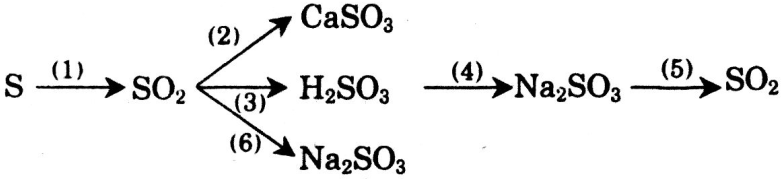
\includegraphics[scale=.3]{S}
	\end{figure}
\end{baitoan}

\begin{proof}[Giải]
	(1) \ce{S + O2 ->[$t^\circ$] SO2}. (2) \ce{SO2 + CaO -> CaSO3} hoặc \ce{SO2 + Ca(OH)2 -> CaSO3 + H2O}. (3) \ce{SO2 + H2O <=> H2SO3}. (4) \ce{Na2O + H2SO3 -> Na2SO3 + H2O} hoặc \ce{H2SO3 + $2$NaOH -> Na2SO3 + $2$H2O}. (5) \ce{Na2SO3 + H2SO4 -> Na2SO4 + H2O + SO2 ^}. (6) \ce{SO2 + $2$NaOH -> Na2SO3 + H2O} hoặc \ce{Na2O + SO2 -> Na2SO3}.
\end{proof}

\begin{baitoan}[\cite{SGK_Hoa_Hoc_9}, 2., p. 11]
	Nhận biết từng chất trong mỗi nhóm chất sau bằng phương pháp hóa học. (a) 2 chất rắn màu trắng {\rm CaO, \ce{P2O5}}. (b) 2 chất khí không màu {\rm\ce{SO2,O2}}. Viết {\rm PTHH}.
\end{baitoan}

\begin{proof}[1st giải]
	(a) Cho nước vào 2 ống nghiệm có chứa CaO \& \ce{P2O5}. Sau đó cho quỳ tím vào mỗi dung dịch. Dung dịch nào làm đổi màu quỳ tím thành xanh là dung dịch base, tương ứng với chất ban đầu là CaO. Dung dịch nào làm đổi màu quỳ tím thành đỏ là dung dịch acid, chất ban đầu là \ce{P2O5}. PTHH: \ce{CaO + H2O -> Ca(OH)2, P2O5 + $3$H2O -> $2$H3PO4}. (b) Lấy mẫu thử từng khí. Lấy quỳ tím ẩm cho vào từng mẫu thử. Mẫu nào làm quỳ tím hóa đỏ là \ce{SO2}, còn lại là \ce{O2}. PTHH: \ce{SO2 + H2O <=> H2SO3}.
\end{proof}

\begin{proof}[2nd giải]
	(a) Cho nước vào 2 ống nghiệm có chứa CaO \& \ce{P2O5}. Sau đó cho phenolphthalein vào mỗi dung dịch. Dung dịch nào hóa hồng là dung dịch base, tương ứng với chất ban đầu là CaO. Dung dịch nào không đổi màu là dung dịch acid, chất ban đầu là \ce{P2O5}. (b) Dẫn lần lượt từng khí vào dung dịch nước vôi trong, nếu có kết tủa xuất hiện thì khí dẫn vào là \ce{SO2}: \ce{SO2 + Ca(OH)2 -> CaSO3 v + H2O}. Nếu không có hiện tượng gì thì khí dẫn vào là khí \ce{O2}. Hoặc có thể đưa que đóm con than hồng vào 2 khí, que đóm sẽ bùng cháy trong khí \ce{O2}.
\end{proof}

\begin{proof}[3rd giải]
	\cite{Ninh_giai_BT_Hoa_Hoc_9}: (a) CaO \& \ce{P2O5} lần lượt là 1 oxide base \& 1 oxide acid. Có thể cho 2 oxide tác dụng với nước ở 2 cốc riêng biệt. Dùng quỳ tím để thử, nếu có màu xanh thì chất ban đầu là CaO. Nếu quỳ chuyển sang màu đỏ thì chất ban đầu là \ce{P2O5}. PTHH: \ce{CaO + H2O -> Ca(OH)2}: dung dịch base (kiềm), \ce{P2O5 + $3$H2O -> $2$H3PO4}: dung dịch acid. (b) \ce{SO2,O2} có thể dùng tàn đóm đỏ để thử \& nhận ra oxygen. Khí còn lại thêm nước cất, lắc, \& thử dung dịch bằng quỳ tím, quỳ tím chuyển sang màu đỏ thì khí ban đầu là \ce{SO2}. PTHH: \ce{SO2 + H2O <=> H2SO3}: dung dịch sulfurous acid.
\end{proof}

\begin{baitoan}[\cite{SGK_Hoa_Hoc_9}, 3., p. 11]
	Có các khí ẩm (khí có lẫn hơi nước): carbon dioxide, hydrogen, oxygen, sulfur dioxide. Khí nào có thể được làm khô bằng calcium oxide? Giải thích.
\end{baitoan}

\begin{proof}[Giải]
	\cite[pp. 10--11]{Ninh_giai_BT_Hoa_Hoc_9}: Nguyên tắc làm khô các chất khí là chất làm khô chỉ giữ lại hơi nước mà không tác dụng với chất được làm khô. CaO là 1 oxide base, chỉ làm khô được: \ce{H2,O2}. CaO không thể làm khô 2 oxide acid \ce{CO2,SO2} vì vi phạm nguyên tắc này. CaO có thể tác dụng với các oxide acid: \ce{CaO + CO2 -> CaCO3, CaO + SO2 -> CaSO3}.
\end{proof}

\begin{baitoan}[\cite{SGK_Hoa_Hoc_9}, 4., p. 11]
	Có 5 chất khí sau: {\rm\ce{CO2,H2,O2,SO2,N2}}. Cho biết chất nào có tính chất sau: (a) nặng hơn không khí. (b) nhẹ hơn không khí. (c) cháy được trong không khí. (d) tác dụng với nước tạo thành dung dịch acid. (e) làm đục nước vôi trong. (f) đổi màu giấy quỳ tím ẩm thành đỏ.
\end{baitoan}

\begin{proof}[Giải]
	(a) Nặng hơn không khí: \ce{CO2,O2,SO2}. (b) Nhẹ hơn không khí: \ce{H2,N2}. (c) Cháy được trong không khí: \ce{H2}. (d) Tác dụng với nước tạo thành dung dịch acid: \ce{CO2,SO2}. (e) Làm đục nước vôi trong: \ce{CO2,SO2}. (f) Đổi màu giấy quỳ tím ẩm thành đỏ: \ce{CO2,SO2}.
\end{proof}

\begin{baitoan}[\cite{SGK_Hoa_Hoc_9}, 5., p. 11]
	Khí lưu huỳnh dioxide được tạo thành từ cặp chất nào sau đây? (a) {\rm\ce{K2SO3,H2SO4}}. (b) {\rm\ce{K2SO4}, HCl}. (c) {\rm\ce{Na2SO3}, NaOH}. (d) {\rm\ce{Na2SO4,CuCl2}}. (e) {\rm\ce{Na2SO3}, NaCl}. Viết PTHH.
\end{baitoan}

\begin{proof}[Giải]
	\ce{SO2} được tạo thành từ cặp chất \ce{K2SO3,H2SO4}: \ce{K2SO3 + H2SO4 -> K2SO4 + H2O + SO2 ^}.
\end{proof}

\begin{baitoan}[\cite{SGK_Hoa_Hoc_9}, 6., p. 11]
	Dẫn {\rm112 mL} khí {\rm\ce{SO2}} (đktc) đi qua {\rm700 mL} dung dịch {\rm\ce{Ca(OH)2}} có nồng độ {\rm0.01M}, sản phẩm là muối calcium sulfite. (a) Viết PTHH. (b) Tính khối lượng các chất sau phản ứng.
\end{baitoan}

\begin{proof}[Giải]
	$n_{\ce{SO2}} = \frac{0.112}{22.4} = 0.005$ mol, $n_{\ce{Ca(OH)2}} = 0.01\cdot0.7 = 0.007$ mol. Vì tỷ số mol $\dfrac{n_{\ce{Ca(OH)2}}}{n_{\ce{SO2}}} = \dfrac{0.007}{0.005} = 1.4 > 1$ nên phản ứng chỉ tạo muối \ce{CaSO3}. (a) PTHH: \ce{SO2 + Ca(OH)2 -> CaSO3 v + H2O} với $n_{\ce{SO2}} = n_{\ce{Ca(OH)2}\footnotesize\mbox{pư}} = n_{\ce{CaSO3}} = 0.005$ mol, $n_{\ce{Ca(OH)2}\footnotesize\mbox{dư}} = 0.007 - 0.005 = 0.002$ mol. (b) $m_{\ce{Ca(OH)2}\footnotesize\mbox{dư}} = 0.002\cdot74 = 0.148$ g, $m_{\ce{CaSO3}} = 0.005\cdot120 = 0.6$ g.
\end{proof}

%------------------------------------------------------------------------------%

\section{Tính Chất Hóa Học của Acid}

\begin{baitoan}[\cite{SGK_Hoa_Hoc_9}, 1., p. 14]
	Từ {\rm Mg, MgO, \ce{Mg(OH)2}} \& dung dịch acid sulfuric loãng, viết các {\rm PTHH} của phản ứng điều chế magnesium sulfate.
\end{baitoan}

\begin{proof}[Giải]
	\ce{Mg + H2SO4 -> MgSO4 + H2 ^, MgO + H2SO4 -> MgSO4 + H2O, Mg(OH)2 + H2SO4 -> MgSO4 + $2$H2O}.
\end{proof}

\begin{baitoan}[\cite{SGK_Hoa_Hoc_9}, 2., p. 14]
	Có các chất sau: {\rm CuO, Mg, \ce{Al2O3,Fe(OH)3,Fe2O3}}. Chọn 1 trong các chất đã cho tác dụng với dung dịch {\rm HCl} sinh ra: (a) khí nhẹ hơn không khí \& cháy được trong không khí. (b) dung dịch có màu xanh lam. (c) dung dịch có màu vàng nâu. (d) dung dịch không có màu. Viết {\rm PTHH}.
\end{baitoan}

\begin{proof}[Giải]
	\cite{Ninh_giai_BT_Hoa_Hoc_9}: (a) Khí nhẹ hơn không khí \& cháy được trong không khí là hydrogen. \ce{Mg + $2$HCl -> MgCl2 + H2 ^}. (b) Dung dịch có màu xanh làm là dung dịch muối copper (II). \ce{CuO + $2$HCl -> CuCl2 + H2O}. (c) Dung dịch có màu vàng nâu: chọn \ce{Fe(OH)3} hoặc \ce{Fe2O3}. \ce{Fe(OH)3 + $3$HCl -> FeCl3 + $3$H2O} hoặc \ce{Fe2O3 + $6$HCl -> $2$FeCl3 + $3$H2O}. (d) Dung dịch không màu: dung dịch \ce{MgCl2} hoặc \ce{AlCl3}. \ce{Mg + $2$HCl -> MgCl2 + H2 ^} hoặc \ce{Al2O3 + $6$HCl -> $2$AlCl3 + $3$H2O}.
\end{proof}

\begin{baitoan}[\cite{SGK_Hoa_Hoc_9}, 3., p. 14]
	Viết {\rm PTHH}: (a) magnesium oxide \& acid nitric. (b) copper {\rm(II)} oxide \& hydrochloric acid. (c) aluminium oxide \& sulfuric acid. (d) iron \& hydrochloric acid. (e) zinc \& sulfuric acid loãng.
\end{baitoan}

\begin{proof}[Giải]
	(a) \ce{MgO + $2$HNO3 -> Mg(NO3)2 + H2O}. (b) \ce{CuO + H2SO4 -> CuSO4 + H2O}. (c) \ce{Al2O3 + $3$H2SO4 -> Al2(SO4)3 + $3$H2O}. (d) \ce{Fe + $2$HCl -> FeCl2 + H2 ^}. (e) \ce{Zn + H2SO4 -> ZnSO4 + H2 ^}.
\end{proof}

\begin{baitoan}[\cite{SGK_Hoa_Hoc_9}, 4., p. 14]
	Có {\rm10 g} hỗn hợp bột 2 kim loại đồng \& sắt. Giới thiệu phương pháp xác định thành phần \% (theo khối lượng) của mỗi kim loại trong hỗn hợp theo: (a) Phương pháp hóa học. Viết PTHH. (b) Phương pháp vật lý. (Biết copper không tác dụng với acid {\rm HCl} \& acid {\rm\ce{H2SO4}} loãng).
\end{baitoan}

\begin{proof}[Giải]
	\cite[p. 12]{Ninh_giai_BT_Hoa_Hoc_9}: (a) Dùng dung dịch hydrochloric acid dư tác dụng với hỗn hợp, chỉ có sắt phản ứng: \ce{Fe + $2$HCl -> FeCl2 + H2 ^}. Lọc, rửa, \& cân chất rắn không tan sẽ biết khối lượng của Cu. Còn lại là Fe. (b) Cho 10 g hỗn hợp bột 2 kim loại vào phía trong 1 tờ giấy A4 gập đôi. Đưa nam châm đến phía ngoài của tờ giấy. Mở tờ giấy ra, sẽ tách riêng bột sắt do nam châm hút \& bột đồng thì không. Cân từng chất.
\end{proof}

%------------------------------------------------------------------------------%

\section{1 Số Acid Quan Trọng}

\begin{baitoan}[\cite{SGK_Hoa_Hoc_9}, 1., p. 19]
	Có các chất: {\rm CuO, \ce{BaCl2}, Zn, ZnO}. Chất nào tác dụng với dung dịch {\rm HCl}, dung dịch {\rm\ce{H2SO4}} loãng sinh ra: (a) chất khí cháy được trong không khí? (b) dung dịch có màu xanh lam? (c) chất kết tủa màu trắng không tan trong nước \& acid? (d) dung dịch không màu \& nước? Viết tất cả các {\rm PTHH}.
\end{baitoan}

\begin{proof}[Giải]
	\cite[p. 13]{Ninh_giai_BT_Hoa_Hoc_9}: (a) Chất khí cháy được trong không khí ở đây chỉ có thể là \ce{H2}. Chỉ có Zn tác dụng với dung dịch acid HCl \& dung dịch \ce{H2SO4} loãng, giải phóng khí \ce{H2}. \ce{Zn + $2$HCl -> ZnCl2 + H2 ^, Zn + H2SO4 -> ZnSO4 + H2 ^}. (b) Dung dịch có màu xanh lam là màu của muối copper (II). \ce{CuO + H2SO4 -> CuSO4 + H2O, CuO + $2$HCl -> CuCl2 + H2O}. (c) Chất kết tủa màu trắng không tan trong nước ở đây là \ce{BaSO4}. \ce{BaCl2 + H2SO4 -> BaSO4 v + $2$HCl}. (d) Dung dịch không màu \& nước là dung dịch \ce{ZnCl2,ZnSO4}. \ce{ZnO + $2$HCl -> ZnCl2 + H2O, ZnO + H2SO4 -> ZnSO4 + H2O}.
\end{proof}

\begin{baitoan}[\cite{SGK_Hoa_Hoc_9}, 2., p. 19]
	Sản xuất acid sulfuric trong công nghiệp cần phải có các nguyên liệu chủ yếu nào? Cho biết mục đích của mỗi công đoạn sản xuất acid sulfuric \& viết {\rm PTHH}.
\end{baitoan}

\begin{proof}[Giải]
	Trong công nghiệp, acid sulfuric được sản xuất bằng \textit{phương pháp tiếp xúc}. Nguyên liệu là sulfur (hoặc quặng pyrit \ce{FeS2}), không khí, \& nước. \textit{Các công đoạn sản xuất acid sulfuric}: Sản xuất sulfur dioxide bằng cách đốt sulfur trong không khí: \ce{S + O2 ->[$t^\circ$] SO2}. Sản xuất sulfur trioxide \ce{SO3} bằng cách oxy hóa \ce{SO2} (chất xúc tác là \ce{V2O5} ở nhiệt độ $450^\circ$C): \ce{$2$SO2 + O2 ->[$t^\circ$][V2O5] $2$SO3}. Sản xuất acid sulfuric bằng cách cho \ce{SO3} tác dụng với nước: \ce{SO3 + H2O -> H2SO4}.
\end{proof}

\begin{baitoan}[\cite{SGK_Hoa_Hoc_9}, 3., p. 19]
	Bằng cách nào có thể nhận biết được từng chất trong mỗi cặp chất sau theo phương pháp hóa học? (a) Dung dịch {\rm HCl} \& dung dịch {\rm\ce{H2SO4}}. (b) Dung dịch {\rm NaCl} \& dung dịch {\rm\ce{Na2SO4}}. (c) Dung dịch {\rm\ce{Na2SO4}} \& dung dịch {\rm\ce{H2SO4}}. Viết {\rm PTHH}.
\end{baitoan}

\begin{proof}[Giải]
	\cite[p. 14]{Ninh_giai_BT_Hoa_Hoc_9}: Lấy 2 ống nghiệm nhỏ, mỗi ống chứa riêng biệt khoảng 1 mL dung dịch chưa biết. (a) Dùng thuốc thử \ce{BaCl2}, nếu chất nào tạo thành kết tủa trắng thì đó là \ce{H2SO4}: \ce{BaCl2 + H2SO4 -> BaSO4 v + $2$HCl}. (b) Dùng thuốc thử \ce{BaCl2}, nếu chất nào tạo thành kết tủa trắng thì đó là \ce{Na2SO4}: \ce{BaCl2 + Na2SO4 -> BaSO4 v + $2$NaCl}. (c) Dùng quỳ tím để thử, nếu quỳ tím chuyển sang màu đỏ thì đó là \ce{H2SO4}.
\end{proof}

\begin{baitoan}[\cite{SGK_Hoa_Hoc_9}, 4., p. 19]
	Bảng sau cho biết kết quả của $6$ thí nghiệm xảy ra giữa {\rm Fe} \& dung dịch {\rm\ce{H2SO4}} loãng. Trong mỗi thí nghiệm người ta dùng {\rm0.2 g Fe} tác dụng với thể tích bằng nhau của acid, nhưng có nồng độ khác nhau.
	\begin{table}[H]
		\centering
		\begin{tabular}{|c|c|c|c|c|}
			\hline
			Thí nghiệm & Nồng độ acid & Nhiệt độ (${}^\circ$C) & Sắt ở dạng & Thời gian phản ứng xong (s) \\
			\hline
			1 & 1M & 25 & Lá & 190 \\
			\hline
			2 & 2M & 25 & Bột & 85 \\
			\hline
			3 & 2M & 35 & Lá & 62 \\
			\hline
			4 & 2M & 50 & Bột & 15 \\
			\hline
			5 & 2M & 35 & Bột & 45 \\
			\hline
			6 & 3M & 50 & Bột & 11 \\
			\hline
		\end{tabular}
	\end{table}
	\noindent Các thí nghiệm nào chứng tỏ: (a) Phản ứng xảy ra nhanh hơn khi tăng nhiệt độ? (b) Phản ứng xảy ra nhanh hơn khi tăng diện tích tiếp xúc? (c) Phản ứng xảy ra nhanh hơn khi tăng nồng độ acid?
\end{baitoan}

\begin{proof}[Giải]
	\cite[p. 15]{Ninh_giai_BT_Hoa_Hoc_9}: Khi xét ảnh hưởng có 1 yếu tố nào đó đến tốc độ phản ứng thì thông thường người ta cố định các yếu tố còn lại, e.g., khi xét ảnh hưởng của yếu tố nhiệt độ, người ta cố định các yếu tố khác như nồng độ acid, diện tích tiếp xúc. (a) Thí nghiệm 2, 4, \& 5. (b) Thí nghiệm 3 \& 5. (c) Thí nghiệm 4 \& 6.
\end{proof}

\begin{baitoan}[\cite{SGK_Hoa_Hoc_9}, 5., p. 19]
	Sử dụng các chất có sẵn: {\rm Cu, Fe, CuO, KOH, \ce{C6H12O6}} (glucose), dung dịch {\rm\ce{H2SO4}} loãng, {\rm\ce{H2SO4}} đặc \& các dụng cụ thí nghiệm cần thiết để làm các thí nghiệm chứng minh: (a) Dung dịch {\rm\ce{H2SO4}} loãng có các tính chất hóa học của acid. (b) {\rm\ce{H2SO4}} đặc có các tính chất hóa học riêng. Viết {\rm PTHH} cho mỗi thí nghiệm.
\end{baitoan}

\begin{proof}[Giải]
	\cite[p. 15]{Ninh_giai_BT_Hoa_Hoc_9}: (a) Dung dịch \ce{H2SO4} loãng có các tính chất hóa học của acid: \ce{$2$KOH + H2SO4 -> K2SO4 + $2$H2O, Fe + H2SO4 -> FeSO4 + H2 ^, CuO + H2SO4 -> CuSO4 + H2O}. (b) Dung dịch \ce{H2SO4} đặc ngoài các tính chất hóa học của acid còn có các tính chất hóa học riêng: \ce{Cu + $2$H2SO4 ->[$t^\circ$] CuSO4 + SO2 ^ + $2$H2O, C6H12O6 ->[H2SO4] $6$C + $6$H2O}.
\end{proof}

\begin{baitoan}[\cite{SGK_Hoa_Hoc_9}, 6., p. 19]
	Cho 1 lượng mạt sắt dư vào {\rm50 mL} dung dịch {\rm HCl}. Phản ứng xong, thu được {\rm3.36 L} khí (đktc). (a) Viết PTHH. (b) Tính khối lượng mạt sắt đã tham gia phản ứng. (c) Tìm nồng độ mol của dung dịch {\rm HCl} đã dùng.
\end{baitoan}

\begin{proof}[Giải]
	(a) PTHH: \ce{Fe + $2$HCl -> FeCl2 + H2 ^}. (b) $n_{\rm Fe} = n_{\ce{H2}} = \dfrac{3.36}{22.4} = 0.15$ mol $\Rightarrow m_{\rm Fe} = 0.15\cdot56 = 8.4$ g. (c) $n_{\rm HCl} = 2n_{\ce{H2}} = 2\cdot0.15 = 0.3$ mol $\Rightarrow C_{\rm M,HCl} =  \dfrac{0.3}{0.05} = 6$M.
\end{proof}

\begin{baitoan}[\cite{SGK_Hoa_Hoc_9}, 7., p. 19]
	Hòa tan hoàn toàn {\rm12.1 g} hỗn hợp bột {\rm CuO, ZnO} cần {\rm100 mL} dung dịch {\rm HCl 3M}. (a) Viết {\rm PTHH}. (b) Tính \% theo khối lượng của mỗi oxide trong hỗn hợp ban đầu. (c) Tính khối lượng dung dịch {\rm\ce{H2SO4}} nồng độ $20\%$ để hòa tan hoàn toàn hỗn hợp các oxide trên.
\end{baitoan}

\begin{proof}[Giải]
	(a) \ce{CuO + $2$HCl -> CuCl2 + H2O, ZnO + $2$HCl -> ZnCl2 + H2O}. (b) Đặt $x\coloneqq n_{\rm CuO}$, $y\coloneqq n_{\rm ZnO}$ trong hỗn hợp. Khối lượng hỗn hợp $m_{\rm hh} = 80x + 81y = 12.1$. Số mol HCl $n_{\rm HCl} = 2(x + y) = 3\cdot0.1 = 0.3$ mol. Giải hệ phương trình
	\begin{equation*}
		\left\{\begin{split}
			80x + 81y &= 12.1,\\
			2(x + y) &= 0.3,
		\end{split}\right.
	\end{equation*}
	được $x = 0.05$ mol, $y = 0.1$ mol. $\%m_{\rm CuO} = \dfrac{0.05\cdot80}{12.1}\cdot100\%\approx33.058\%$, $\%m_{\rm ZnO} = \dfrac{0.1\cdot81}{12.1}\cdot100\%\approx66.942\%$ (hoặc $\%m_{\rm ZnO} = 100\% - \%m_{\rm CuO}\approx100\% - 33.058\% = 66.942\%$). (c) \ce{CuO + H2SO4 -> CuSO4 + H2O, ZnO + H2SO4 -> ZnSO4 + H2O}. $n_{\ce{H2SO4}} = n_{\rm CuO} + n_{\rm ZnO} = 0.05 + 0.1 = 0.15$ mol $\Rightarrow m_{\ce{H2SO4}} = 98\cdot0.15 = 14.7$ g $\Rightarrow m_{dd\ce{H2SO4}} = \frac{14.7}{20\%} = 73.5$ g.
\end{proof}

%------------------------------------------------------------------------------%

\section{Luyện Tập: Tính Chất Hóa Học của Oxide \& Acid}

\begin{baitoan}[\cite{SGK_Hoa_Hoc_9}, 1., p. 21]
	Có các oxide: {\rm\ce{SO2,CuO,Na2O,CO2}}. Cho biết các oxide nào tác dụng được với: (a) nước. (b) hydrochloric acid. (c) sodium hydroxide. Viết {\rm PTHH}.
\end{baitoan}

\begin{proof}[Giải]
	(a) Oxide tác dụng với nước: \ce{SO2,Na2O,CaO,CO2}. \ce{SO2 + H2O <=> H2SO3, Na2O + H2O -> $2$NaOH, CaO + H2O -> Ca(OH)2, CO2 + H2O <=> H2CO3}. (b) Oxide tác dụng với hydrochloric acid: \ce{Na2O}, CaO. \ce{Na2O + $2$HCl -> $2$NaCl + H2O, CaO + $2$HCl -> CaCl2 + H2O}. (c) Oxide tác dụng với sodium hydroxide: \ce{SO2,CO2}. \ce{SO2 + $2$NaOH -> Na2SO3 + H2O, CO2 + $2$NaOH -> Na2CO3 + H2O}.
\end{proof}

\begin{baitoan}[\cite{SGK_Hoa_Hoc_9}, 2., p. 21]
	Các oxide nào sau: {\rm\ce{H2O,CuO,Na2O,CO2,P2O5}} có thể điều chế bằng: (a) phản ứng hóa hợp? Viết PTHH. (b) phản ứng hóa hợp \& phản ứng phân hủy? Viết PTHH.
\end{baitoan}

\begin{proof}[Giải]
	(a) Oxide được điều chế bằng phản ứng hóa hợp: \ce{H2O,Na2O,P2O5}. \ce{$2$H2 + O2 -> $2$H2O, $4$Na + O2 -> $2$Na2O, $4$P + $5$O2 -> $2$P2O5}. (b) Oxide được điều chế bằng phản ứng hóa hợp \& phân hủy: CuO, \ce{CO2}. \ce{$2$Cu + O2 -> $2$CuO, Cu(OH)2 ->[$t^\circ$] CuO + H2O, C + O2 -> CO2, CaCO3 ->[$t^\circ$] CaO + CO2 ^}.
\end{proof}

\begin{baitoan}[\cite{SGK_Hoa_Hoc_9}, 3., p. 21]
	Khí {\rm CO} được dùng làm chất đốt trong công nghiệp, có lẫn tạp chất là các khí {\rm\ce{CO2,SO2}}. Làm thế nào có thể loại bỏ được các tạp chất ra khỏi {\rm CO} bằng hóa chất rẻ tiền nhất? Viết {\rm PTHH}.
\end{baitoan}

\begin{proof}[Giải]
	 Sử dụng calcium hydroxide dư để loại bỏ \ce{CO2,SO2} bằng cách sục hỗn hợp khí chưa sạch qua bình rửa khí chứa \ce{Ca(OH)2} bởi vì \ce{Ca(OH)2} là chất kiềm rẻ nhất. \ce{CO2 + Ca(OH)2 -> CaCO3 v + H2O, SO2 + Ca(OH)2 -> CaSO3 v + H2O}.
\end{proof}

\begin{baitoan}[\cite{SGK_Hoa_Hoc_9}, 4., p. 21]
	Cần phải điều chế 1 lượng muối copper {\rm(II)} sulfate. Phương pháp nào sau đây tiết kiệm được acid sulfuric? (a) Acid sulfuric tác dụng với copper {\rm(II)} oxide. (b) Acid sulfuric đặc tác dụng với kim loại đồng. Vì sao?
\end{baitoan}

\begin{proof}[Giải]
	(a) \ce{CuO + H2SO4 -> CuSO4 + H2O}. (b) \ce{Cu + $2$H2SO4 \mbox{đặc} ->[$t^\circ$] CuSO4 + $2$H2O + SO2 ^}. So sánh 2 phương trình, ta thấy để điều chế cùng 1 lượng muối copper (II) sulfate như nhau, cách thứ nhất tiết kiệm acid sulfuric hơn.
\end{proof}

\begin{baitoan}[\cite{SGK_Hoa_Hoc_9}, 5., p. 21]
	Thực hiện các chuyển đổi hóa học sau bằng cách viết các {\rm PTHH} (ghi điều kiện của phản ứng, nếu có):
	\begin{figure}[H]
		\centering
		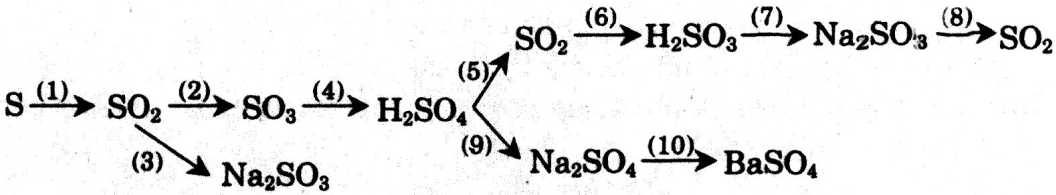
\includegraphics[scale=.8]{S1}
	\end{figure}
\end{baitoan}

\begin{proof}[Giải]
	(1) \ce{S + O2 -> SO2}. (2) \ce{$2$SO2 + O2 ->[$t^\circ$][V2O5] $2$SO3}. (3) \ce{SO2 + $2$NaOH -> Na2SO3 + H2O}. (4) \ce{SO3 + H2O -> H2SO4}. (5) \ce{Cu + $2$H2SO4 \mbox{đặc} ->[$t^\circ$] CuSO4 + $2$H2O + SO2 ^}. (6) \ce{SO2 + H2O -> H2SO3}. (7) \ce{H2SO3 + $2$NaOH -> Na2SO3 + $2$H2O}. (8) \ce{Na2SO3 + H2SO4 -> Na2SO4 + H2O + SO2 ^}. (9) \ce{H2SO4 + $2$NaOH -> Na2SO4 + $2$H2O}. (10) \ce{Na2SO4 + BaCl2 -> BaSO4 v + $2$NaCl}.
\end{proof}

%------------------------------------------------------------------------------%

\section{Tính Chất Hóa Học của Base}

\begin{baitoan}[\cite{SGK_Hoa_Hoc_9}, 1., p. 25]
	Có phải tất cả các chất kiềm đều là base không? Dẫn ra CTHH của 3 chất kiềm để minh họa. Có phải tất cả các base đều là chất kiềm không? Dẫn ra {\rm CTHH} của các base để minh họa.
\end{baitoan}

\begin{proof}[Giải]
	Base chia thành 2 loại, base tan trong nước thành dung dịch gọi là \textit{kiềm} \& base không tan. Base kiềm, e.g., NaOH, KOH, \ce{Ca(OH)2,Ba(OH)2}, $\ldots$ Base không tan, e.g., \ce{Fe(OH)2,Fe(OH)3,Cu(OH)2}, $\ldots$
\end{proof}

\begin{baitoan}[\cite{SGK_Hoa_Hoc_9}, 2., p. 25]
	Có 3 base sau: {\rm\ce{Cu(OH)2,NaOH,Ba(OH)2}}. Cho biết các base nào: (a) tác dụng được với dung dịch {\rm HCl}. (b) bị nhiệt phân hủy. (c) tác dụng được với {\rm\ce{CO2}}. (d) đổi màu quỳ tím thành xanh. Viết {\rm PTHH}.
\end{baitoan}

\begin{proof}[Giải]
	(a) Cả 3 base đều tác dụng được với HCl: \ce{Cu(OH)2 + $2$HCl -> CuCl2 + $2$H2O, Ba(OH)2 + $2$HCl -> BaCl2 + $2$H2O, NaOH + HCl -> NaCl + H2O}. (b) Bị nhiệt phân hủy chỉ gồm các base không tan: \ce{Cu(OH)2 ->[$t^\circ$] CuO + H2O}. (c) Tác dụng được với \ce{CO2} chỉ gồm các kiềm: \ce{CO2 + Ba(OH)2 -> BaCO3 v + H2O, CO2 + $2$NaOH -> Na2CO3 + H2O}. (d) Đổi màu quỳ tím thành xanh là tính chất riêng của kiềm: NaOH, \ce{Ba(OH)2}.
\end{proof}

\begin{baitoan}[\cite{SGK_Hoa_Hoc_9}, 3., p. 25]
	Từ các chất có sẵn: {\rm\ce{Na2O,CaO,H2O}}. Viết {\rm PTHH} điều chế các dung dịch base.
\end{baitoan}

\begin{proof}[Giải]
	(a) Điều chế các dung dịch base từ oxide base tương ứng tác dụng với nước: \ce{Na2O + H2O -> $2$NaOH, CaO + H2O -> Ca(OH)2}. (b) Điều chế các base không tan từ muối tương ứng tác dụng với kiềm: \ce{CuCl2 + $2$NaOH -> $2$NaCl + Cu(OH)2 v, FeCl3 + $3$NaOH -> $3$NaCl + Fe(OH)3 v}.
\end{proof}

\begin{baitoan}[\cite{SGK_Hoa_Hoc_9}, 4., p. 25]
	Có 4 lọ không nhãn, mỗi lọ đựng 1 dung dịch không màu sau: {\rm NaCl, \ce{Ba(OH)2}, NaOH, \ce{Na2SO4}}. Chỉ được dùng quỳ tím, làm thế nào nhận biết dung dịch đựng trong mỗi lọ bằng phương pháp hóa học? Viết {\rm PTHH}.
\end{baitoan}

\begin{proof}[Giải]
	\cite[p. 20]{Ninh_giai_BT_Hoa_Hoc_9}: Lấy 4 ống nghiệm, lấy mỗi chất vào từng ống nghiệm, đánh số thứ tự các ống \& thử theo các bước sau. \textit{Bước 1}: Nhỏ dung dịch của 4 chất này vào 1 mẩu quỳ tím. Nếu quỳ tím hóa xanh thì đó là 2 kiềm: \ce{Ba(OH)2} \& NaOH. Nếu quỳ tím không đổi màu thì đó là NaCl \& \ce{Na2SO4}. \textit{Bước 2}: Lấy 2 dung dịch kiềm đổ lần lượt vào 2 lọ còn lại, nếu thấy xuất hiện kết tủa thì đó là dung dịch \ce{Ba(OH)2} \& \ce{Na2SO4}: \ce{Ba(OH)2 + Na2SO4 -> BaSO4 v + $2$NaOH}. \textit{Bước 3}: Nhận biết được dung dịch kiềm còn lại là NaOH \& muối còn lại là NaCl.
\end{proof}

\begin{baitoan}[\cite{SGK_Hoa_Hoc_9}, 4., p. 25]
	Cho {\rm15.5 g} sodium oxide {\rm\ce{Na2O}} tác dụng với nước, thu được {\rm0.5 L} dung dịch base. (a) Viết {\rm PTHH} \& tính nồng độ mol của dung dịch base thu được. (b) Tính thể tích dung dịch {\rm\ce{H2SO4} 20\%}, có khối lượng riêng {\rm1.14 g{\tt/}mL} cần dùng để trung hòa dung dịch base nói trên.
\end{baitoan}

\begin{proof}[Giải]
	(a) \ce{Na2O + H2O -> $2$NaOH} với $n_{\ce{Na2O}} = \dfrac{15.5}{62} = 0.25$ mol, $n_{\rm NaOH} = 2n_{\ce{Na2O}} = 2\cdot0.25 = 0.5$ mol. $C_{\rm M,NaOH} = \dfrac{0.5}{0.5} = 1$M. (b) \ce{H2SO4 + $2$NaOH -> Na2SO4 + $2$H2O}. $n_{\ce{H2SO4}} = \frac{1}{2}n_{\rm NaOH} = \dfrac{0.5}{2} = 0.25$ mol $\Rightarrow m_{\ce{H2SO4}} = 0.25\cdot98 = 24.5$ g. Khối lượng dung dịch \ce{H2SO4} $20\%$: $m_{\rm dd\ce{H2SO4}} = \dfrac{24.5}{20\%} = 122.5$ g. Thể tích dung dịch \ce{H2SO4} $20\%$: $V_{\rm dd\ce{H2SO4}} = \dfrac{122.5}{1.14}\approx107.456$ mL.
\end{proof}

%------------------------------------------------------------------------------%

\section{1 Số Base Quan Trọng}

\begin{baitoan}[\cite{SGK_Hoa_Hoc_9}, 1., p. 27]
	Có 3 lọ không nhãn, mỗi lọ đựng 1 chất rắn sau: {\rm NaOH, NaCl, \ce{Ba(OH)2}}. Trình bày cách nhận biết chất đựng trong mỗi lọ bằng phương pháp hóa học. Viết {\rm PTHH} (nếu có).
\end{baitoan}

\begin{baitoan}[\cite{SGK_Hoa_Hoc_9}, 2., p. 27]
	Có các chất: {\rm Zn, \ce{Zn(OH)2,NaOH,Fe(OH)3,CuSO4}, NaCl, HCl}. Chọn chất thích hợp điền vào mỗi sơ đồ phản ứng sau \& lập PTHH: {\rm(a) $\ldots$ \ce{->[$t^\circ$] Fe2O3 + H2O}. (b) \ce{H2SO4 + $\ldots$ -> Na2SO4 + H2O}. (c) \ce{H2SO4 + $\ldots$ -> ZnSO4 + H2O}. (d) \ce{NaOH + $\ldots$ -> NaCl + H2O}. (e) $\ldots$ \ce{+ CO2 -> Na2CO3 + H2O}}.
\end{baitoan}

\begin{baitoan}[\cite{SGK_Hoa_Hoc_9}, 1., p. 30]
	Viết {\rm PTHH} thực hiện các chuyển đổi hóa học: (a) {\rm\ce{CaCO3} $\to$ CaO $\to$ \ce{Ca(OH)2} $\to$ \ce{CaCO3}}. (b) {\rm CaO $\to$ \ce{CaCl2}}. (c) {\rm\ce{Ca(OH)2} $\to$ \ce{Ca(NO3)2}}.
\end{baitoan}

\begin{baitoan}[\cite{SGK_Hoa_Hoc_9}, 2., p. 30]
	Có 3 lọ không nhãn, mỗi lọ đựng 1 trong 3 chất rắn màu trắng: {\rm\ce{CaCO3,Ca(OH)2}, CaO}. Nhận biết chất đựng trong mỗi lọ bằng phương pháp hóa học. Viết {\rm PTHH}.
\end{baitoan}

\begin{baitoan}[\cite{SGK_Hoa_Hoc_9}, 3., p. 30]
	Viết {\rm PTHH} của phản ứng khi dung dịch {\rm NaOH} tác dụng với dung dịch {\rm\ce{H2SO4}} tạo ra: (a) muối sodium hydrosunfate. (b) muối sodium sulfate.
\end{baitoan}

\begin{baitoan}[\cite{SGK_Hoa_Hoc_9}, 4., p. 30]
	1 dung dịch bão hòa khí {\rm\ce{CO2}} trong nước có $\rm pH = 4$. Giải thích \& viết {\rm PTHH} của {\rm\ce{CO2}} với nước.
\end{baitoan}

\begin{baitoan}[\cite{SGK_Hoa_Hoc_9}, 7.1., p. 9]
	Nêu các tính chất hóa học giống \& khác nhau của base tan (kiềm) \& base không tan. Dẫn ra ví dụ, viết PTHH.
\end{baitoan}

\begin{baitoan}[\cite{SGK_Hoa_Hoc_9}, 7.2., p. 9]
	Các base khi bị nung nóng tạo ra oxide là: {\sf A.} {\rm\ce{Mg(OH)2,Cu(OH2),Zn(OH)2,Fe(OH)3}}. {\sf B.} {\rm\ce{Ca(OH)2,Al(OH)3}, KOH, NaOH}. {\sf C.} {\rm\ce{Zn(OH)2,Mg(OH)2,Fe(OH)3}, KOH}. {\sf D.} {\rm\ce{Fe(OH)3,Al(OH)3,Zn(OH)2}, NaOH}.
\end{baitoan}

\begin{baitoan}[\cite{SGK_Hoa_Hoc_9}, 7.3., p. 9]
	Dung dịch {\rm HCl}, khí {\rm\ce{CO2}} đều tác dụng với: {\sf A.} {\rm\ce{Ca(OH)2,Ba(OH)2}, NaOH, KOH}. {\sf B.} {\rm\ce{Ca(OH)2,Al(OH)3}, KOH, NaOH}. {\sf C.} {\rm NaOH, KOH, \ce{Fe(OH)3, Ba(OH)3}}. {\sf D.} {\rm\ce{Ca(OH)2,Cr(OH)3}, KOH}.
\end{baitoan}

\begin{baitoan}[\cite{SGK_Hoa_Hoc_9}, 7.4., p. 9]
	Viết CTHH của các: (a) base ứng với các oxide: {\rm\ce{Na2O,Al2O3,Fe2O3}, BaO}. (b) oxide ứng với các base: {\rm KOH, \ce{Ca(OH)2,Zn(OH)2,Cu(OH)2}}.
\end{baitoan}

\begin{baitoan}[\cite{SGK_Hoa_Hoc_9}, 7.5., p. 9]
	Có 3 lọ không nhãn, mỗi lọ đựng 1 trong các chất rắn: {\rm\ce{Cu(OH)2,Ba(OH)2,Na2CO3}}. Chọn 1 thuốc thử để có thể nhận biết được cả 3 chất này. Viết {\rm PTHH}.
\end{baitoan}

\begin{baitoan}[\cite{SGK_Hoa_Hoc_9}, 8.1., p. 9]
	Bằng phương pháp hóa học nào có thể phân biệt được 2 dung dịch base: {\rm NaOH, \ce{Ca(OH)2}}? Viết PTHH.
\end{baitoan}

\begin{baitoan}[\cite{SGK_Hoa_Hoc_9}, 8.2., p. 9]
	Có 4 lọ không nhãn, mỗi lọ đựng 1 trong các dung dịch sau: {\rm NaOH, \ce{Na2SO4,H2SO4}, HCl}. Nhận biết dung dịch trong mỗi lọ bằng phương pháp hóa học. Viết {\rm PTHH}.
\end{baitoan}

\begin{baitoan}[\cite{SGK_Hoa_Hoc_9}, 8.3., p. 10]
	Cho các chất: {\rm\ce{Na2CO3,Ca(OH)2}, NaCl}. (a) Từ các chất đã cho, viết các {\rm PTHH} điều chế {\rm NaOH}. (b) Nếu các chất đã cho có khối lượng bằng nhau, ta dùng phản ứng nào để có thể điều chế được khối lượng {\rm NaOH} nhiều hơn?
\end{baitoan}

\begin{baitoan}[\cite{SGK_Hoa_Hoc_9}, 8.4., p. 10]
	Bảng sau cho biết giá trị pH của dung dịch 1 số chất:
	\begin{table}[H]
		\centering
		\begin{tabular}{|c|c|c|c|c|c|}
			\hline
			Dung dịch & A & B & C & D & E \\
			\hline
			pH & 13 & 3 & 1 & 7 & 8 \\
			\hline
		\end{tabular}
	\end{table}
	\noindent(a) Dự đoán trong các dung dịch trên: (1) Dung dịch nào có thể là acid, e.g., {\rm HCl, \ce{H2SO4}}? (2) Dung dịch nào có thể là base, e.g., {\rm NaOH, \ce{Ca(OH)2}}? (3) Dung dịch nào có thể là đường, muối {\rm NaCl}, nước cất? (4) Dung dịch nào có thể là acid acetic (có trong giấm ăn)? (5) Dung dịch nào có tính base yếu, e.g., {\rm\ce{NaHCO3}}? (b) Cho biết: (1) Dung dịch nào có phản ứng với {\rm Mg}, với {\rm NaOH}? (2) Dung dịch nào có phản ứng với dung dịch {\rm HCl}? (3) Các dung dịch nào trộn với nhau từng đôi một sẽ xảy ra phản ứng hóa học?	
\end{baitoan}

\begin{baitoan}[\cite{SGK_Hoa_Hoc_9}, 3., p. 27]
	Dẫn từ từ {\rm1.568 L} khí {\rm\ce{CO2}} (đktc) vào 1 dung dịch có hòa tan {\rm6.4 g NaOH}, sản phẩm là muối {\rm\ce{Na2CO3}}. (a) Chất nào đã lấy dư \& dư là bao nhiêu ({\rm L} hoặc {\rm g})? (b) Tính khối lượng muối thu được sau phản ứng.
\end{baitoan}

\begin{baitoan}[\cite{SGK_Hoa_Hoc_9}, 8.5., p. 10]
	{\rm3.04 g} hỗn hợp {\rm NaOH, KOH} tác dụng vừa đủ với dung dịch {\rm HCl}, thu được {\rm4.15 g} các muối clorua. (a) Viết {\rm PTHH}. (b) Tính khối lượng của mỗi hydroxide trong hỗn hợp ban đầu.
\end{baitoan}

\begin{baitoan}[\cite{SGK_Hoa_Hoc_9}, 8.6., p. 10]
	Cho {\rm10 g \ce{CaCO3}} tác dụng với dung dịch {\rm HCl} dư. (a) Tính thể tích khí {\rm\ce{CO2}} thu được ở đktc. (b) Dẫn khí {\rm\ce{CO2}} thu được ở trên vào lọ đựng {\rm50 g} dung dịch {\rm NaOH 40\%}. Tính khối lượng muối carbonate thu được.
\end{baitoan}

\begin{baitoan}[\cite{SGK_Hoa_Hoc_9}, 8.7., p. 10]
	Cho $m$ {\rm g} hỗn hợp gồm {\rm\ce{Mg(OH)2,Cu(OH)2}, NaOH} tác dụng vừa đủ với {\rm400 mL} dung dịch {\rm HCl 1M} \& tạo thành {\rm24.1 g} muối clorua. Tính $m$.
\end{baitoan}

\begin{baitoan}[\cite{SGK_Hoa_Hoc_9}, 1., p. 33]
	Dẫn ra 1 dung dịch muối khi tác dụng với 1 dung dịch chất khác thì tạo ra: (a) chất khí. (b) chất kết tủa. Viết {\rm PTHH}.
\end{baitoan}

\begin{baitoan}[\cite{SGK_Hoa_Hoc_9}, 2., p. 33]
	Có 3 lọ không nhãn, mỗi lọ đựng 1 dung dịch muối sau: {\rm\ce{CuSO4,AgNO3}, NaCl}. Dùng các dung dịch có sẵn trong phòng thí nghiệm để nhận biết chất đựng trong mỗi lọ. Viết {\rm PTHH}.
\end{baitoan}

\begin{baitoan}[\cite{SGK_Hoa_Hoc_9}, 3., p. 33]
	Có các dung dịch muối: {\rm\ce{Mg(NO3)2,CuCl2}}. Cho biết muối nào có thể tác dụng với: (a) Dung dịch {\rm NaOH}. (b) Dung dịch {\rm HCl}. (c) Dung dịch {\rm\ce{AgNO3}}. Nếu có phản ứng, viết các PTHH.
\end{baitoan}

\begin{baitoan}[\cite{SGK_Hoa_Hoc_9}, 4., p. 33]
	Cho các dung dịch muối sau phản ứng với nhau từng đôi một, viết dấu $\cdot$ nếu có phản ứng \& viết PTHH, dấu $\circ$ nếu không.
\end{baitoan}

\begin{baitoan}[\cite{SGK_Hoa_Hoc_9}, 5., p. 33]
	Ngâm 1 đinh sắt sạch trong dung dịch copper {\rm(II)} sulfate. Câu trả lời nào sau đây là đúng nhất cho hiện tượng quan sát được? {\sf A.} không có hiện tượng nào xảy ra. {\sf B.} Kim loại đồng màu đỏ bám ngoài đinh sắt, đinh sắt không có sự thay đổi. {\sf C.} 1 phần đinh sắt bị hòa tan, kim loại đồng bám ngoài đinh sắt \& màu xanh lam của dung dịch ban đầu nhạt dần. {\sf D.} Không có chất mới nào được sinh ra, chỉ có 1 phần đinh sắt bị hòa tan. Giải thích cho sự lựa chọn \& viết PTHH, nếu có.
\end{baitoan}

\begin{baitoan}[\cite{SGK_Hoa_Hoc_9}, 1., p. 36]
	Cho các muối: {\rm\ce{CaCO3,CaSO4,Pb(NO3)2}, NaCl}. Muối nào nói trên: (a) không được phép có trong nước ăn vì tính độc hại của nó? (b) không độc nhưng cũng không nên có trong nước ăn vì vị mặn của nó? (c) không tan trong nước, nhưng bị phân hủy ở nhiệt độ cao? (d) rất ít tan trong nước \& khó bị phân hủy ở nhiệt độ cao?
\end{baitoan}

\begin{baitoan}[\cite{SGK_Hoa_Hoc_9}, 2., p. 36]
	2 dung dịch tác dụng với nhau, sản phẩm thu được có {\rm NaCl}. Cho biết 2 dung dịch chất ban đầu có thể là các chất nào. Minh họa bằng các PTHH.
\end{baitoan}

\begin{baitoan}[\cite{SGK_Hoa_Hoc_9}, 3., p. 36]
	(a) Viết phương trình điện phân dung dịch muối ăn (có màng ngăn). (b) Các sản phẩm của sự điện phân dung dịch {\rm NaCl} có nhiều ứng dụng quan trọng: Khí clo dùng để: $\ldots$ Khí hydrogen dùng để: $\ldots$. Sodium hydroxide dùng để: $\ldots$ Điền các ứng dựng sau vào các chỗ trống cho phù hợp: tẩy trắng vải, giấy; nấu xà phòng; sản xuất hydrochloric acid; chế tạo hóa chất trừ sâu, diệt cỏ dại; hàn cắt kim loại; sát trùng, diệt khuẩn nước ăn; nhiên liệu cho động cơ tên lửa; bơm khí cầu, bóng thám không; sản xuất nhôm, sản xuất chất dẻo PVC; chế biến dầu mỏ.
\end{baitoan}

\begin{baitoan}[\cite{SGK_Hoa_Hoc_9}, 4., p. 36]
	Dung dịch {\rm NaOH} có thể dùng để phân biệt 2 muối có trong mỗi cặp chất sau được không? (a) Dung dịch {\rm\ce{K2SO4}} \& dung dịch {\rm\ce{Fe2(SO4)3}}. (b) Dung dịch {\rm\ce{Na2SO4}} \& dung dịch {\rm\ce{CuSO4}}. (c) Dung dịch {\rm NaCl} \& dung dịch {\rm\ce{BaCl2}}. Viết {\rm PTHH}, nếu có.
\end{baitoan}

\begin{baitoan}[\cite{SGK_Hoa_Hoc_9}, 6., p. 33]
	Trộn {\rm30 mL} dung dịch có chứa {\rm2.22 g \ce{CaCl2}} với {\rm70 mL} dung dịch có chứa {\rm1.7 g \ce{AgNO3}}. (a) Cho biết hiện tượng quan sát được \& viết PTHH. (b) Tính khối lượng chất rắn sinh ra. (c) Tính nồng độ mol của chất còn lại trong dung dịch sau phản ứng. Cho thể tích của dung dịch thay đổi không đáng kể.
\end{baitoan}

\begin{baitoan}[\cite{SGK_Hoa_Hoc_9}, 5., p. 36]
	Trong phòng thí nghiệm có thể dùng các muối {\rm\ce{KClO3}} hoặc {\rm\ce{KNO3}} để điều chế khí oxygen bằng phản ứng phân hủy. (a) Viết {\rm PTHH}. (b) Nếu dùng {\rm0.1 mol} mỗi chất thì thể tích khí oxygen thu được có khác nhau không? Tính thể tích khí oxygen thu được. (c) Cần điều chế {\rm1.12 L} khí oxygen, tính khối lượng mỗi chất cần dùng. Các thể tích khí được đo ở đktc.
\end{baitoan}

\begin{baitoan}[\cite{SGK_Hoa_Hoc_9}, 1., p. 39]
	Có các loại phân bón hóa học: {\rm KCl, \ce{NH4NO3, NH4Cl, (NH4)2SO4, Ca3(PO4)2, Ca(H2PO4)2}, \ce{(NH4)2HPO4, KNO3}}. (a) Cho biết tên hóa học của các phân bón này. (b) Sắp xếp các phân bón này thành 2 nhóm phân bón đơn \& phân bón kép. (c) Trộn các phân bón nào với nhau ta được phân bón kép NPK?
\end{baitoan}

\begin{baitoan}[\cite{SGK_Hoa_Hoc_9}, 2., p. 39]
	Có 3 mẫu phân bón hóa học không ghi nhãn: phân kali {\rm KCl}, phân đạm {\rm\ce{NH4NO3}} \& phân supephotphat (phân lân) {\rm\ce{Ca(H2PO4)2}}. Nhận biết mỗi mẫu phân bón trên băng phương pháp hóa học.
\end{baitoan}

\begin{baitoan}[\cite{SGK_Hoa_Hoc_9}, 3., p. 39]
	1 người làm vườn đã dùng {\rm500 g \ce{(NH4)2SO4}} để bón rau. (a) Nguyên tố dinh dưỡng nào có trong loại phân bón này? (b) Tính thành phần \% của nguyên tố dinh dưỡng trong phân bón. (c) Tính khối lượng của nguyên tố dinh dưỡng bón cho ruộng rau.
\end{baitoan}

%------------------------------------------------------------------------------%

\section{Salt -- Muối}

%------------------------------------------------------------------------------%

\section{Phân Bón Hóa Học}

%------------------------------------------------------------------------------%

\section{Mối Quan Hệ Giữa Các Loại Hợp Chất Vô Cơ}

\begin{baitoan}[\cite{SGK_Hoa_Hoc_9}, 1., p. 41]
	Chất nào trong các thuốc thử sau có thể dùng để phân biệt dung dịch sodium sulfate \& dung dịch sodium carbonate? (a) Dung dịch barium chloride. (b) Dung dịch hydrochloric acid. (c) Dung dịch chì nitrate. (d) Dung dịch bạc nitrate. (e) Dung dịch sodium hydroxide. Giải thích \& viết các PTHH.
\end{baitoan}

\begin{baitoan}[\cite{SGK_Hoa_Hoc_9}, 2., p. 41]
	Cho các dung dịch sau lần lượt phản ứng với nhau từng đôi một, ghi $1$ nếu có phản ứng, $0$ nếu không có phản ứng. Viết {\rm PTHH} nếu có.
	\begin{table}[H]
		\centering
		\begin{tabular}{|c|c|c|c|}
			\hline
			& NaOH & HCl & \ce{H2SO4} \\
			\hline
			\ce{CuSO4} &  &  &  \\
			\hline
			HCl &  &  &  \\
			\hline
			\ce{Ba(OH)2} &  &  &  \\
			\hline
		\end{tabular}
	\end{table}
\end{baitoan}

\begin{baitoan}[\cite{SGK_Hoa_Hoc_9}, 4., p. 41]
	Có các chất: {\rm\ce{Na2O}, Na, NaOH, \ce{Na2SO4,Na2CO3}, NaCl}. (a) Dựa vào mối quan hệ giữa các chất, sắp xếp các chất trên thành 1 dãy chuyển đổi hóa học. (b) Viết {\rm PTHH} cho dãy chuyển đổi hóa học ở (a).
\end{baitoan}

\begin{baitoan}[\cite{SGK_Hoa_Hoc_9}, 2., p. 43]
	Để 1 mẩu sodium hydroxide trên tấm kính trong không khí, sau vài ngày thấy có chất rắn màu trắng phủ ngoài. Nếu nhỏ vài giọt dung dịch {\rm HCl} vào chất rắn trắng thấy có khí thoát ra, khí này làm đục nước vôi trong. Chất rắn màu trắng là sản phẩm phản ứng của sodium hydroxide với chất nào sau đây? Giải thích \& viết {\rm PTHH} minh họa. (a) Oxygen trong không khí. (b) Hơi nước trong không khí. (c) Carbon dioxide \& oxygen trong không khí. (d) Carbon dioxide \& hơi nước trong không khí. (e) Carbon dioxide trong không khí.
\end{baitoan}

\begin{baitoan}[\cite{SGK_Hoa_Hoc_9}, 3., p. 43]
	Trộn 1 dung dịch có hòa tan {\rm0.2 mol \ce{CuCl2}} với 1 dung dịch có hòa tan {\rm20 g NaOH}. Lọc hỗn hợp các chất sau phản ứng, được kết tủa \& nước lọc. Nung kết tủa đến khi khối lượng không đổi. (a) Viết {\rm PTHH}. (b) Tính khối lượng chất rắn thu được sau khi nung. (c) Tính khối lượng các chất tan có trong nước lọc.
\end{baitoan}

%------------------------------------------------------------------------------%

\printbibliography[heading=bibintoc]

\end{document}